\documentclass[a4paper,10pt]{article}
\usepackage[utf8]{inputenc}			%encodage
\usepackage[T1]{fontenc}
\usepackage[french]{babel}
				%Mise en page
%\usepackage{layout}				%Affichage du gabarit de la page
\usepackage[top=0.5 in, bottom=0.5 in, left=0.5 in, right=0.5 in]{geometry}				%Modification des marges
\usepackage{geometry}				%Modification des marges
%\usepackage{setspace}				%Interligne
%\usepackage{soul}				%Barrer le texte
%\usepackage{ulem}				%Sous-ligner
%\usepackage{eurosym}				%Signe euro
%\usepackage{fancyhdr}
%\pagestyle{fancy}
%\usepackage{geometry}
%\geometry{top=3cm, bottom=3cm, left=3cm , right=0.5cm}
				%Pack de polices
%\usepackage{bookman}                    
%\usepackage{charter}
%\usepackage{newcent}
%\usepackage{lmodern}
%\usepackage{mathpazo}
%\usepackage{mathptmx}
				%Suite
%\usepackage{url}				%Cr\'{e}ation d'url
\usepackage{verbatim}				%Citation de code
%\usepackage{moreverb}				%Citation de code
\usepackage{listings}				%Citation de code color\'{e}
%\usepackage{fancyhdr}				%En tete et pied de page personnalis\'{e}
%\usepackage{multicol}				%Pouvoir ecrire sur plusieures colonnes
				%Figures
\usepackage{graphicx}				%Travailler avec des images
%\usepackage{wrapfig}				%Seulement en dernier recours
				%Couleur
%\usepackage{color}				%Colorer le texte 

%\usepackage{colortbl}				%Colorer les tableaux
				%Maths
%\usepackage{amsthm}				%Th\'{e}orèmes
\usepackage{amsmath}
%\usepackage{amssymb}
%\usepackage{mathrsfs}
				%Cr\'{e}ation d'index
%\usepackage{makeidx}
				%Creation d'arbres
%\usepackage{tikz}
\usepackage{enumitem}     %listings alphanum\'{e}iques
\usepackage{hyperref}
%\usepackage{minted}

% Title Page
\title{Projet Noté\\
\large\emph{Algorithmes Avancés}}
\author{José Ferro Pinto\and Fabrice Ceresa}
%\setcounter{section}{-1}

\begin{document}
\maketitle

\section{Partie 1}  
    \subsection{Valeur optimale pour K}
        Nous avons utilisé la méthode des K-Means avec un nombre de clusters K qui varie entre 1 et 25 et comme paramètres : \verb?init='random'? pour que l’algorithme choisisse comme barycentres initiaux des données aléatoires et \verb?random_state=0? comme seed pour le générateur de nombres aléatoires.
        
        Pour chaque valeur de K, nous avons déterminé la moyenne des distances moyennes entre les barycentres et leurs points. Nous obtenons comme résultats:
        
        \begin{center}
            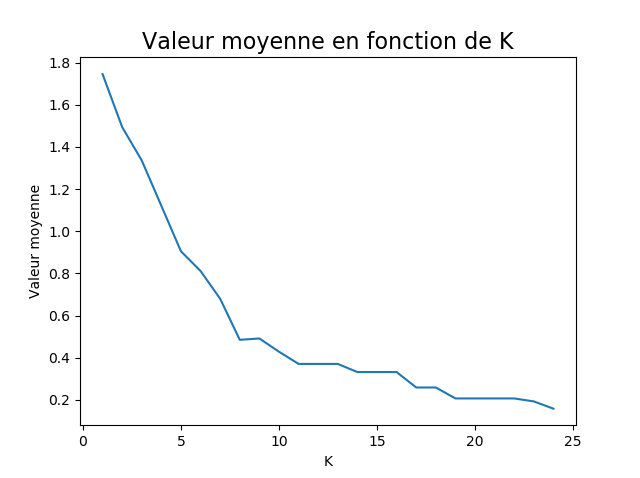
\includegraphics{p1-1}
        \end{center}
        
        Nous pouvons voir que le nombre optimal de clusters à choisir est 8.
        
        \pagebreak
        
        En effet, plus K augmente plus la valeur moyenne diminue mais on peut voir qu’à partir de K = 8 la distance entre les barycentres et leurs points diminue beaucoup moins vite. Choisir un nombre de clusters plus élevé n’apporterait donc pas beaucoup plus d’information sur les données.
        
        Représentation des données :
        
        \begin{center}
            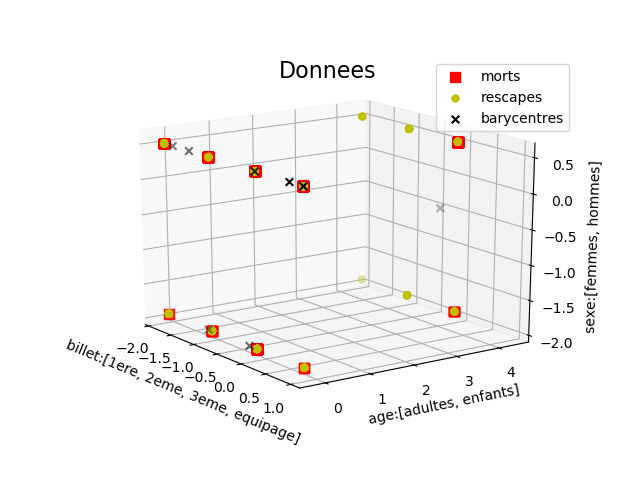
\includegraphics{p1-2}
        \end{center}
        
        A partir de la représentation en 3 dimensions, nous pouvons déjà constater qu’aucun enfant en 1ère et 2ème classes n’est mort et que le sexe n’a que peu d’influence sur le taux de survie des enfants.
        
        \begin{center}
            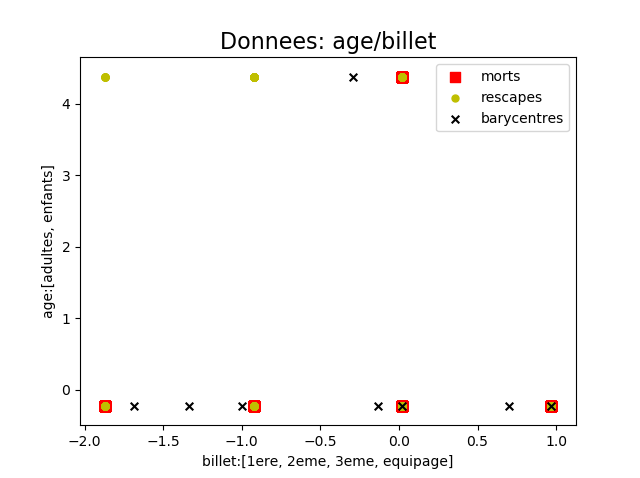
\includegraphics{p1-3}
        \end{center}
        
        Nous pouvons voir par la position des barycentres que la grande majorité des passagers étaient des adultes et que parmi eux la plupart étaient en 3ème classe ou faisaient partie de l’équipage. C’est dans ces groupes que se trouvaient la majeure partie des personnes qui n’ont pas survécu.
        
        \begin{center}
            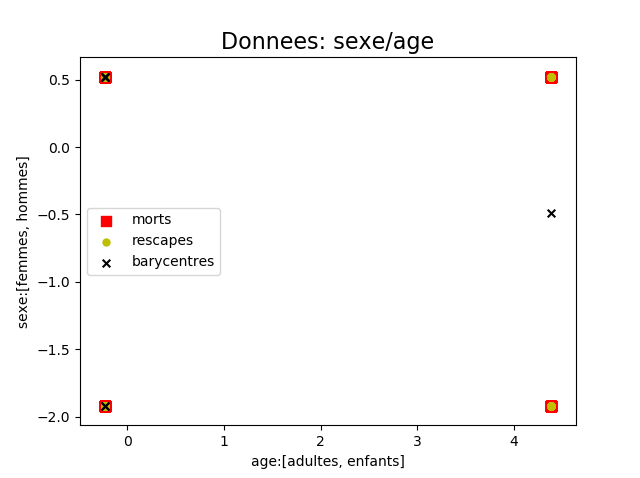
\includegraphics{p1-4}
        \end{center}
        
        Ici nous constatons (mieux avec la représentation 3d) qu’il y avait bien plus d’hommes que de femmes sur le Titanic et que leur taux de survie était plus faible.
        
        \begin{center}
            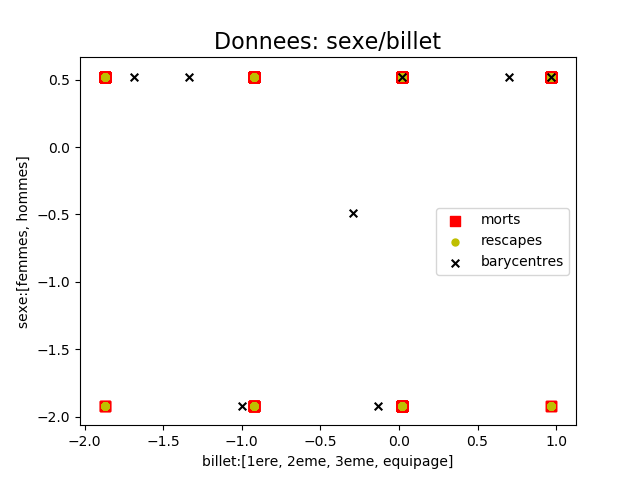
\includegraphics{p1-5}
        \end{center}
        
        Finalement ici, nous pouvons voir que les femmes étaient presque pas présentes parmi les membres de l’équipage. C’est surtout le fait d’être une femme qui offrait une meilleure chance de survie mais aussi le fait d’être en 1ère ou 2ème classe. 
\section{Partie 2}
    Pour normaliser les données, nous avons utilisé \verb?preprocessing.normalize(raw['data'])? comme demandé dans le TP.
    
    Le programme se passe en 4 boucles intriquées :
    \begin{enumerate}
        \item Pour chacun des datasets
        \item Pour chacun des classificateurs
        \item Pour chacun des paramètres
        \item Pour chacune des étapes de la validation croisée
    \end{enumerate}
    
    Les datasets utilisés : 
    \begin{itemize}
        \item \verb?load_breast_cancer? pour les données du cancer du sein
        \item \verb?load_wine? pour les données sur du vin
    \end{itemize}
    
    Les différents classificateurs utilisés et leurs paramètres:
    \begin{itemize}
        \item \verb?KNeighborsClassifier? pour la méthode des K-plus proches voisins.
        
        Paramètre variable : \verb?n_neighbors? nombre de voisins pris en compte : [1,51] avec un pas de 5
        \item \verb?DecisionTreeClassifier? pour les arbres de décisions. 
        
        Paramètre variable: \verb?min_samples_leaf? Nombre d'objets à partir duquel on comptabilise une feuille [2, 52] avec un pas de 5
        \item \verb?MLPClassifier? pour le Perceptron multi-couche avec une couche utilisant ``stochastic gradient descent''
        
        Paramètres fixes : \verb?solver='sgd', activation='logistic', max_iter=1000, verbose=False, learning_rate_init=0.1, tol=0., early_stopping=True?
        
        Paramètre variable : \verb?hidden_layer_sizes=(nodes,)? donc une couche et nodes varie entre 2 et 20 par pas de 3.
        \item \verb?MLPClassifier? pour le Perceptron multi-couche avec une couche utilisant ``a stochastic gradient-based optimizer''
        
        Paramètres fixes : \verb?solver='adam', activation='logistic', max_iter=1000, verbose=False, learning_rate_init=0.1, tol=0., early_stopping=True?
        
        Paramètre variable : \verb?hidden_layer_sizes=(nodes,)? donc une couche et nodes varie entre 2 et 20 par pas de 3.
        \item \verb?MLPClassifier? pour le Perceptron multi-couche avec deux couches utilisant ``stochastic gradient descent''
        
        Paramètres fixes : \verb?solver='sgd', activation='logistic', max_iter=1000, verbose=False, learning_rate_init=0.1, tol=0., early_stopping=True?
        
        Paramètre variable : \verb?hidden_layer_sizes=(nodes,)? donc une couche et nodes varie entre 2 et 20 par pas de 3.
        \item \verb?MLPClassifier? pour le Perceptron multi-couche avec deux couches utilisant ``a stochastic gradient-based optimizer''
        
        Paramètres fixes : \verb?solver='adam', activation='logistic', max_iter=1000, verbose=False, learning_rate_init=0.1, tol=0., early_stopping=True?
        
        Paramètre variable : \verb?hidden_layer_sizes=(nodes,)? donc une couche et nodes varie entre 2 et 20 par pas de 3.  
    \end{itemize}
    
    La validation est donc la validation croisée : \verb?RepeatedKFold?
    
    Nous avons décidé de prendre les mesures suivantes :
    \begin{itemize}
        \item le temps d'exécution
        \item la moyenne des scores
        \item l'écart type des scores
    \end{itemize}
    
    La sortie de l'exécution du script python donne la sortie suivante : 
    
    \verbatiminput{partie2.txt}
    
    On peut voir qu'avec un échantillon plus grand (17070 échantillons) on trouve des résultats plus probants qu'avec moins d'échantillons (2314) avec un score moyen général de 0.830857845 avec un écart-type moyen général de 0.011719923 pour le cancer du sein contre 0.565530503 avec un écart-type moyen général moyen de 0.033507676 pour le vin.
    
    Pour ce qui est du temps de travail en fonction du nombre d'échantillons, c'est globalement plus rapide avec moins d'échantillons.
    
    Par contre, c'est pas parce que le temps de travail est plus grand que le score final sera meilleur.
\section{Partie 3}

\end{document}
